\documentclass{article}
\usepackage[utf8]{inputenc}

\title{MSP Temps et évolution chimique : cinétique et catalyse}
\author{Maria Ubero Gonzalez}
\date{Mars 2020}

\usepackage{natbib}
\usepackage{graphicx}
\usepackage{amsmath}
\usepackage[a4paper, total={6in, 8in}]{geometry}
\usepackage{xcolor}
\usepackage{chemist}

\begin{document}

\maketitle

\subsubsection*{BO TS}

\begin{center}
    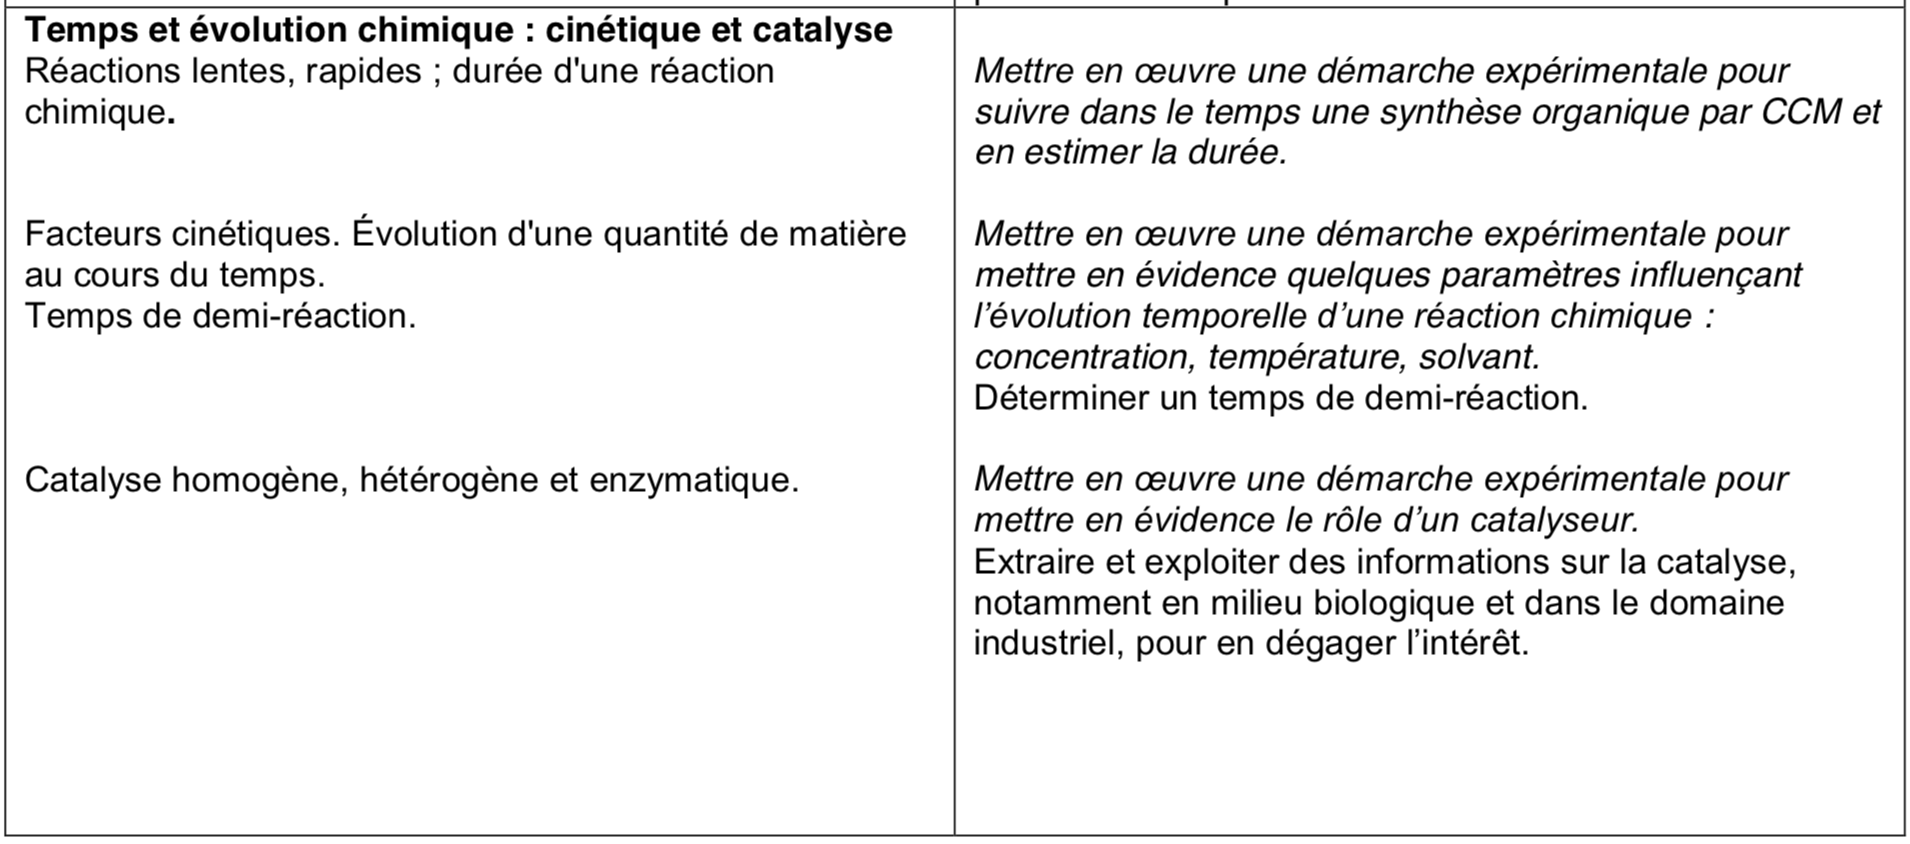
\includegraphics[scale=0.4]{BOcatalyseTS.png}
\end{center}

\subsubsection*{BO 1ere STL spécialité}

\begin{center}
    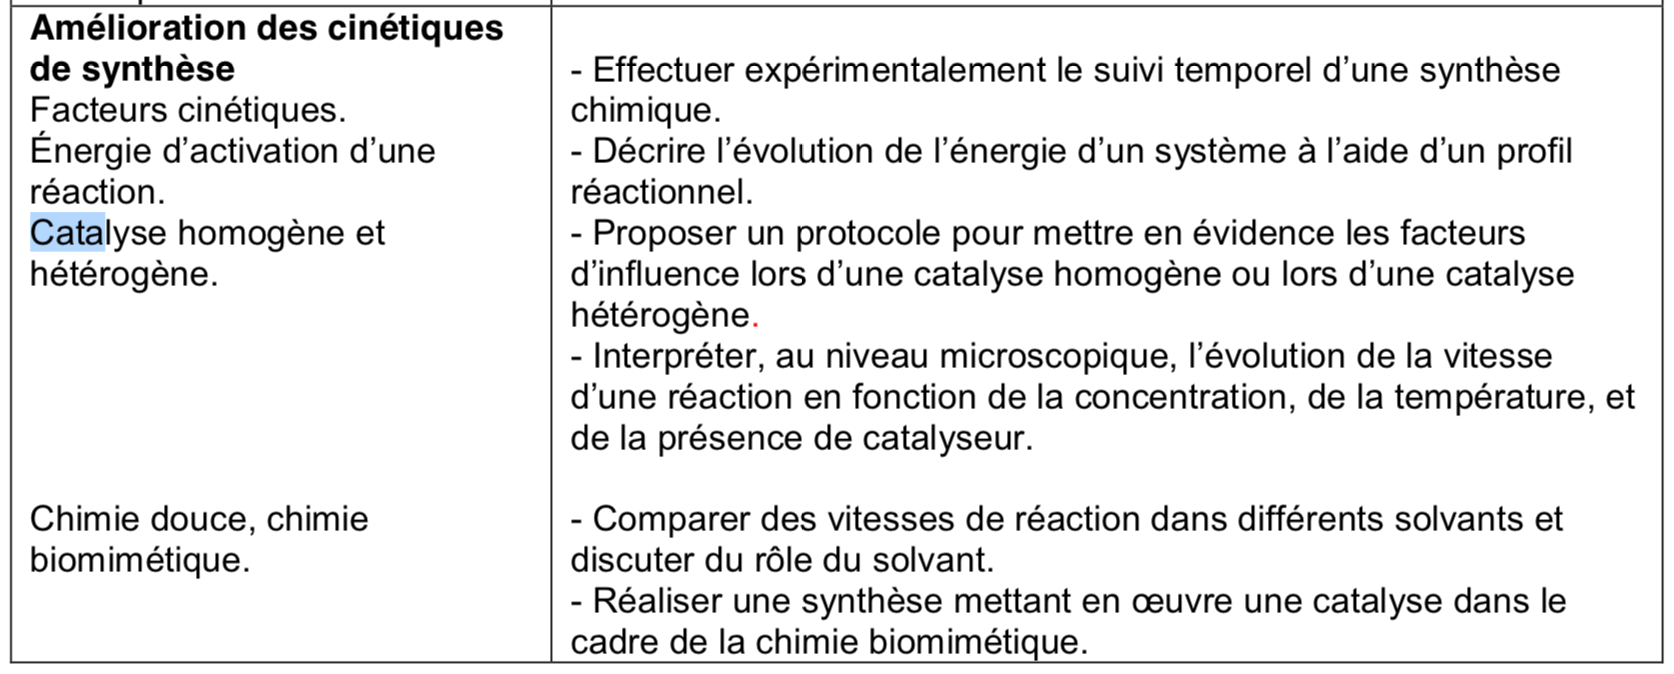
\includegraphics[scale=0.45]{BO 1 STL.png}
\end{center}

\textcolor{blue}{A avoir en tête la cinétique de première année de prépa pour les questions!!!!}

\section*{Pré-requis}


\begin{itemize}
        \item Réactif limitant, tableau d'avancement, stoechiométrie
        \item Synthèse
        \item Oxydo-réduction
\end{itemize}


\textcolor{red}{Manips:}

\begin{itemize}
    \item Quantitative : Spectro UV suivi de l'absorvance.
    \item Qualitatives :
    \begin{itemize}
        \item Décomposition des ions thiosulfate en milieu acide
        \item Réaction entre ions permanganate et l'acide oxalique
        \item Décomposition du peroxyde d'hydrogène en présence des ions $Fe^{3+}$, du platine et du navet(enzyme).
    \end{itemize}
\end{itemize}


\section*{Introduction}

Jusqu'à présent, nous avons écrit que des équations bilan pour modéliser les réactions chimiques. Celles-ci nous renseignent sur les réactifs consommés et les produits formés, mais ne donnent aucune information quant à la rapidité de la transformation chimique qui se déroule. Le facteur temps est absent de la modélisation.\\

La cinétique chimique étudie l'évolution temporelle des systèmes chimiques. Cette discipline a une grande importance dans le milieu industriel, où l'on souhaite produire beaucoup en un minimum de temps et aussi dans l'étude des mécanismes des réaction. C'est un paramètre macroscopique qui nous informe sur le deroulement microscopique d'une réaction :\\

\begin{itemize}
    \item Certaines réactions chimiques paraissent immédiates, c'est le cas d'un grand nombre de réactuions de dosage, que l'on souhaite rapides. \textcolor{red}{Manip}. Verser du permanganate de potassium acidifié dans une solution d'ions \chemform{Fe^{2+}}, la couleur fuschia disparaît instantanément.
    \item Plus lente (quelque minutes) \textcolor{red}{Manip}. Verser du permanganate de potassium acidifié dans une solution d'acide oxalique \chemform{H_2 C_2 O_4}, disparition lente de la couleur fuschia.
    \item Très lentes, des jours ou des années, comme la formation de la rouille (Annexe).
\end{itemize}

Comment modéliser l'évolution temporelle d'une réaction chimique ? Peut-on influer sur cette évolution pour accélérer une réaction désirée, ou ralentir voir bloquer une réaction indésirable ? Nous allons répondre à ces questions durant cette leçon.\\



\section{Evolution temporelle d'un système chimique}
\subsection{Modélisation}

Pour caractériser l'évolution d'un système chimique nous pouvons adopter plusieurs approches :
\begin{itemize}
    \item suivre la diminution de la quantité de matière d'un réactif au cours du temps
    \item suivre l'augmentation de la quantité de matière d'un produit au cours du temps
    \item suivre l'avancement de la réaction au cours du temps.
\end{itemize}

Par exemple (j'utilise cet exemple car je vais en avoir besoin pour la manip quantitative) nous étudions la réaction entre les ions iodure et l'eau oxygénée qu'on peut supposer totale ($E^{\circ} (I_2 / I^{-}) = 0.54 V$ et $E^{\circ} (H_2 O_2 / H_2O) = 1.78)$) :

\begin{chemmath}
    H_2 O_{2(aq)} + 3I^{-}_{(aq)} + 2H^{+}_{(aq)} = I_{3(aq)}^- + 2 H_2 O_{(l)}
\end{chemmath}

Tableau d'avancement :\\

\begin{center}
\begin{tabular}{| l | c | c | c | c | c | }
\hline
    & $H_2 O_{2(aq)}$ & $3I^{-}_{aq}$ & $2H^{+}_{(aq)}$ & $I_{3(aq)}^-$ & $2 H_2 O_l$ \\ \hline
  EI & $n_0$ & $n_1$ & excès & / & / \\ \hline
  EF & $n_0 - \xi$ & $n_1 - 3\xi$ & excès & $\xi$ & $/$ \\ \hline
 \end{tabular}
\end{center}


On voit que connaître la quantité de matière d'une suele espèce permet de déterminer l'avancement pourvu qu'on connaise la composition initiale, et donc la quantité de matière de toutes les autres espèces ayant réagi. Suivre l'avancement en fonction du temps nous permet donc de connaître à tout instant la composition du milieu réactionnel.

\subsection{Méthode de suivi de l'avancement}

Pour suivre une réaction cinétiquement on peut utiliser :

\begin{itemize}
    \item Un suivi \textbf{qualitatif}. Par exemple lorqu'au cours de la réaction on détecte un dégagement gazeux, un changement de couleur, la formation ou la disparition d'un solide. En d'autres termes, un phénomène flagrant, bien repérable. Cela permet de savoir à vue d'oeil quand la réaction est terminée.
    \item \textbf{Quantitativement}. On mesure une grandeur physique reliée à l'avancement de la réaction. Par exemple :
    \begin{itemize}
        \item La conductivité (ions formés ou consommés)
        \item Absorbance, par spectroscopie UV-visible si des espèces absorbant dans le visible (colorées).
        \item RMN. On peut faire des acquisitions tous les minutes, ou tous les heures. On peut tracer la concentration en fonction du temps. Avantage : on peut fixer la température à l'intérieur du spectromètre.
    \end{itemize}
\end{itemize}

\subsubsection*{\textcolor{red}{Manip}. Suivi spectrophotométrique de la formation du diiode Maréchal pag 271}

L'espèce qui absorbe c'est l'ion triiode de couleur jaune orangée. On utilise la loi de Beer-Lambert pour relier la concentration ou la quantité de matière de l'ion triiodure à l'absorbance.

\begin{equation}
    A = k_{\lambda}[I_3^-]
\end{equation}

où $k_{\lambda}$ dépend du spectrophotomètre.\\

\textbf{Définir le temps de demi-réaction avec la manip !!}. On peut le définir en disant que : pour des réactions lentes, il est compliqué de savoir à quel moment la réaction est terminée (dificil à repérer sur la courbe qu'on vient de trouver, on peut le montrer avec regressi avec un pointeur sur la courbe, c'est pour cette raison qu'on défini le temps de demi-réaction.

\subsection{Temps de demi-réaction}

\textbf{Le temps de demi-réaction,} noté $t_{1/2}$ est la durée au terme de laquelle l'avancement $x(t_{1/2})$ de la réaction est égal à la moitié de l'avancement final $x_f$. On considère que l'état final du système est atteint au bout de 6-7 fois le temps de demi-réaction. Ce dernier est donc caractéristique de l'évolution temporelle du système considéré.\medskip

Insister sur le point : à $t=2t_{1/2}$ l'expérience n'est pas finie car l'évolutions de la quantité de matière n'est pas linéaire avec le temps !.\\

\textbf{Calculer le temps de demi-réaction avec la manip proposée}.\\

\textcolor{red}{Intérêt.} Le temps de demi réaction permet de comparer la rapidité des différents réactions (c'est une convencion car pas toutes les réactions sont totales). En plus, pour des réactions lentes, il est compliqué de savoir à quel moment la réaction est terminée (dificil à repérer sur la courbe, on peut le montrer avec regressi avec la courbe qu'on a obtenue precédement, c'est pour cette raison aussi qu'on défini le temps de demi-réaction.)  

\section{Facteurs cinétiques}

Nous venons de voir comment caractériser la rapidité d'une réaction mais, est-ce qu'on peut rendre une réaction rapide ou lente ? La reponse est oui. Nous pouvons jouer sur certains facteurs comme :

\subsection{Influence de la concentration}

\textcolor{violet}{On aurait pu faire comme manip aussi : changer la concentration de $KI$ dans la manip quantitative et montrer que le temps $t_{1/2}$ change (si la concentration augmente, le temps diminue). Pareil pour la température, on aurait pu augmenter la température et voir que le $t_{1/2}$ a diminué. C'est ce que Hugo fait dans sa leçon.}\\

\textcolor{red}{Manip qualitative}. \textbf{Décomposition des ions thiosulfate en milieu acide. Pag 182-183. Sarrazin ou pag 230 TS Hachette.}\\

On prend 2 béchers, on fait une croix sur une feuille blanche qu'on met en dessous de ces béchers pour repérer le moment où on ne peut plus voir ces croix. On prend du thiosulfate à $c = 0,25 mol/L$ et de l'acide chlorydrique à $c=1 mol/L$ (je ne suis pas le protocole du livre de TS).

\begin{itemize}
    \item Bécher 1: 30 mL d'eau, 20 mL de thiosulfate et 5 mL  d'HCl (environ 1 minute)
    \item Bécher 2: 10 mL d'eau, 40 mL de thiosulfate et 5 mL  d'HCl (environ 25 sec)
\end{itemize}

\textbf{Conclusion}. Plus la concentration des réactifs est grande, plus la réaction est rapide.\\

\textcolor{red}{Jeter le milieu réactionnel le plus rapide dans un bécher poubelle contenant de l'eau et quelques pastilles de soude, pour dégrader le dioxyde de soufre toxique libéré par la réaction.}

\begin{center}
    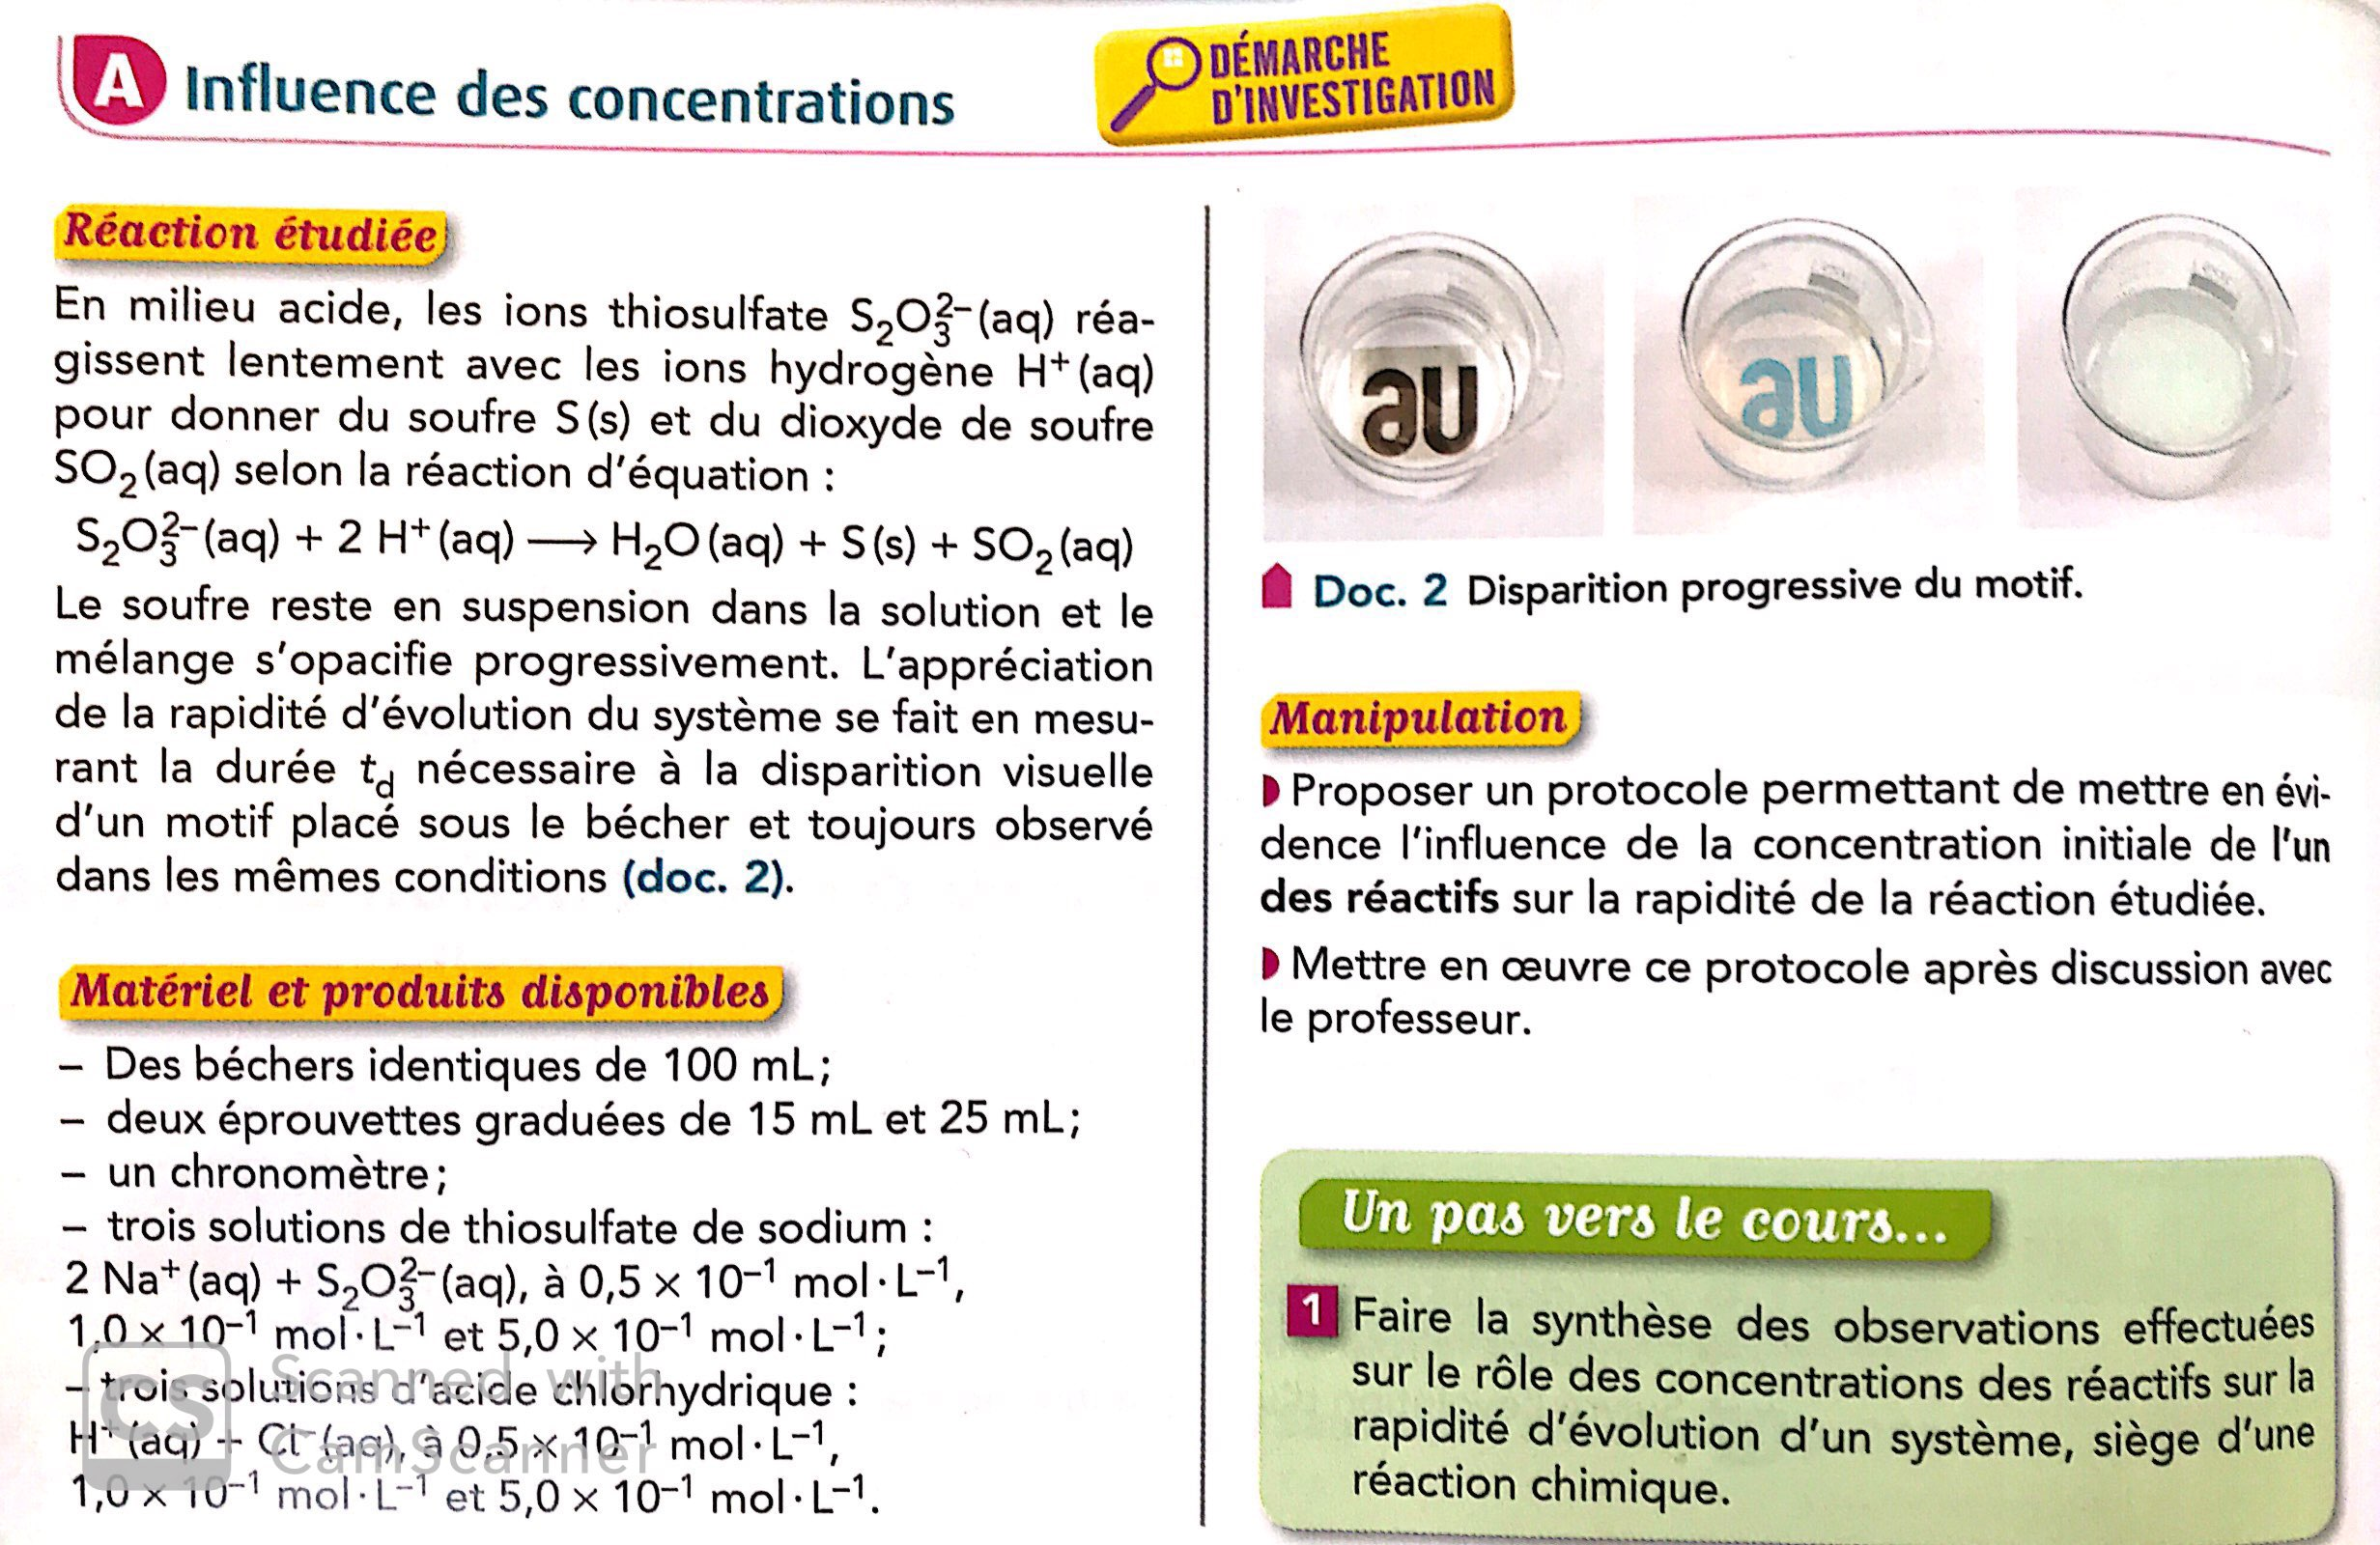
\includegraphics[scale=0.14]{influenceconc.jpg}
\end{center}

\subsection{Influence de la température}

Avoir en tête la loi d'Arhenius !!! Augmenter de 10 degrés augmente k d'un ordre 2.

\textcolor{red}{Manip qualitative}. \textbf{Pag 231 livre TS Hachette} Influence de la température, réaction entre les ions permanganate et l'acide oxalique. On reprend la manip de l'introduction où on a vu que la réaction entre les ions permanganate et l'acide oxalique était lente. Manip qualitative. On prepare un bain-marie à environ $50^{\circ}$ et on prepare aussi de la glace.

\begin{center}
    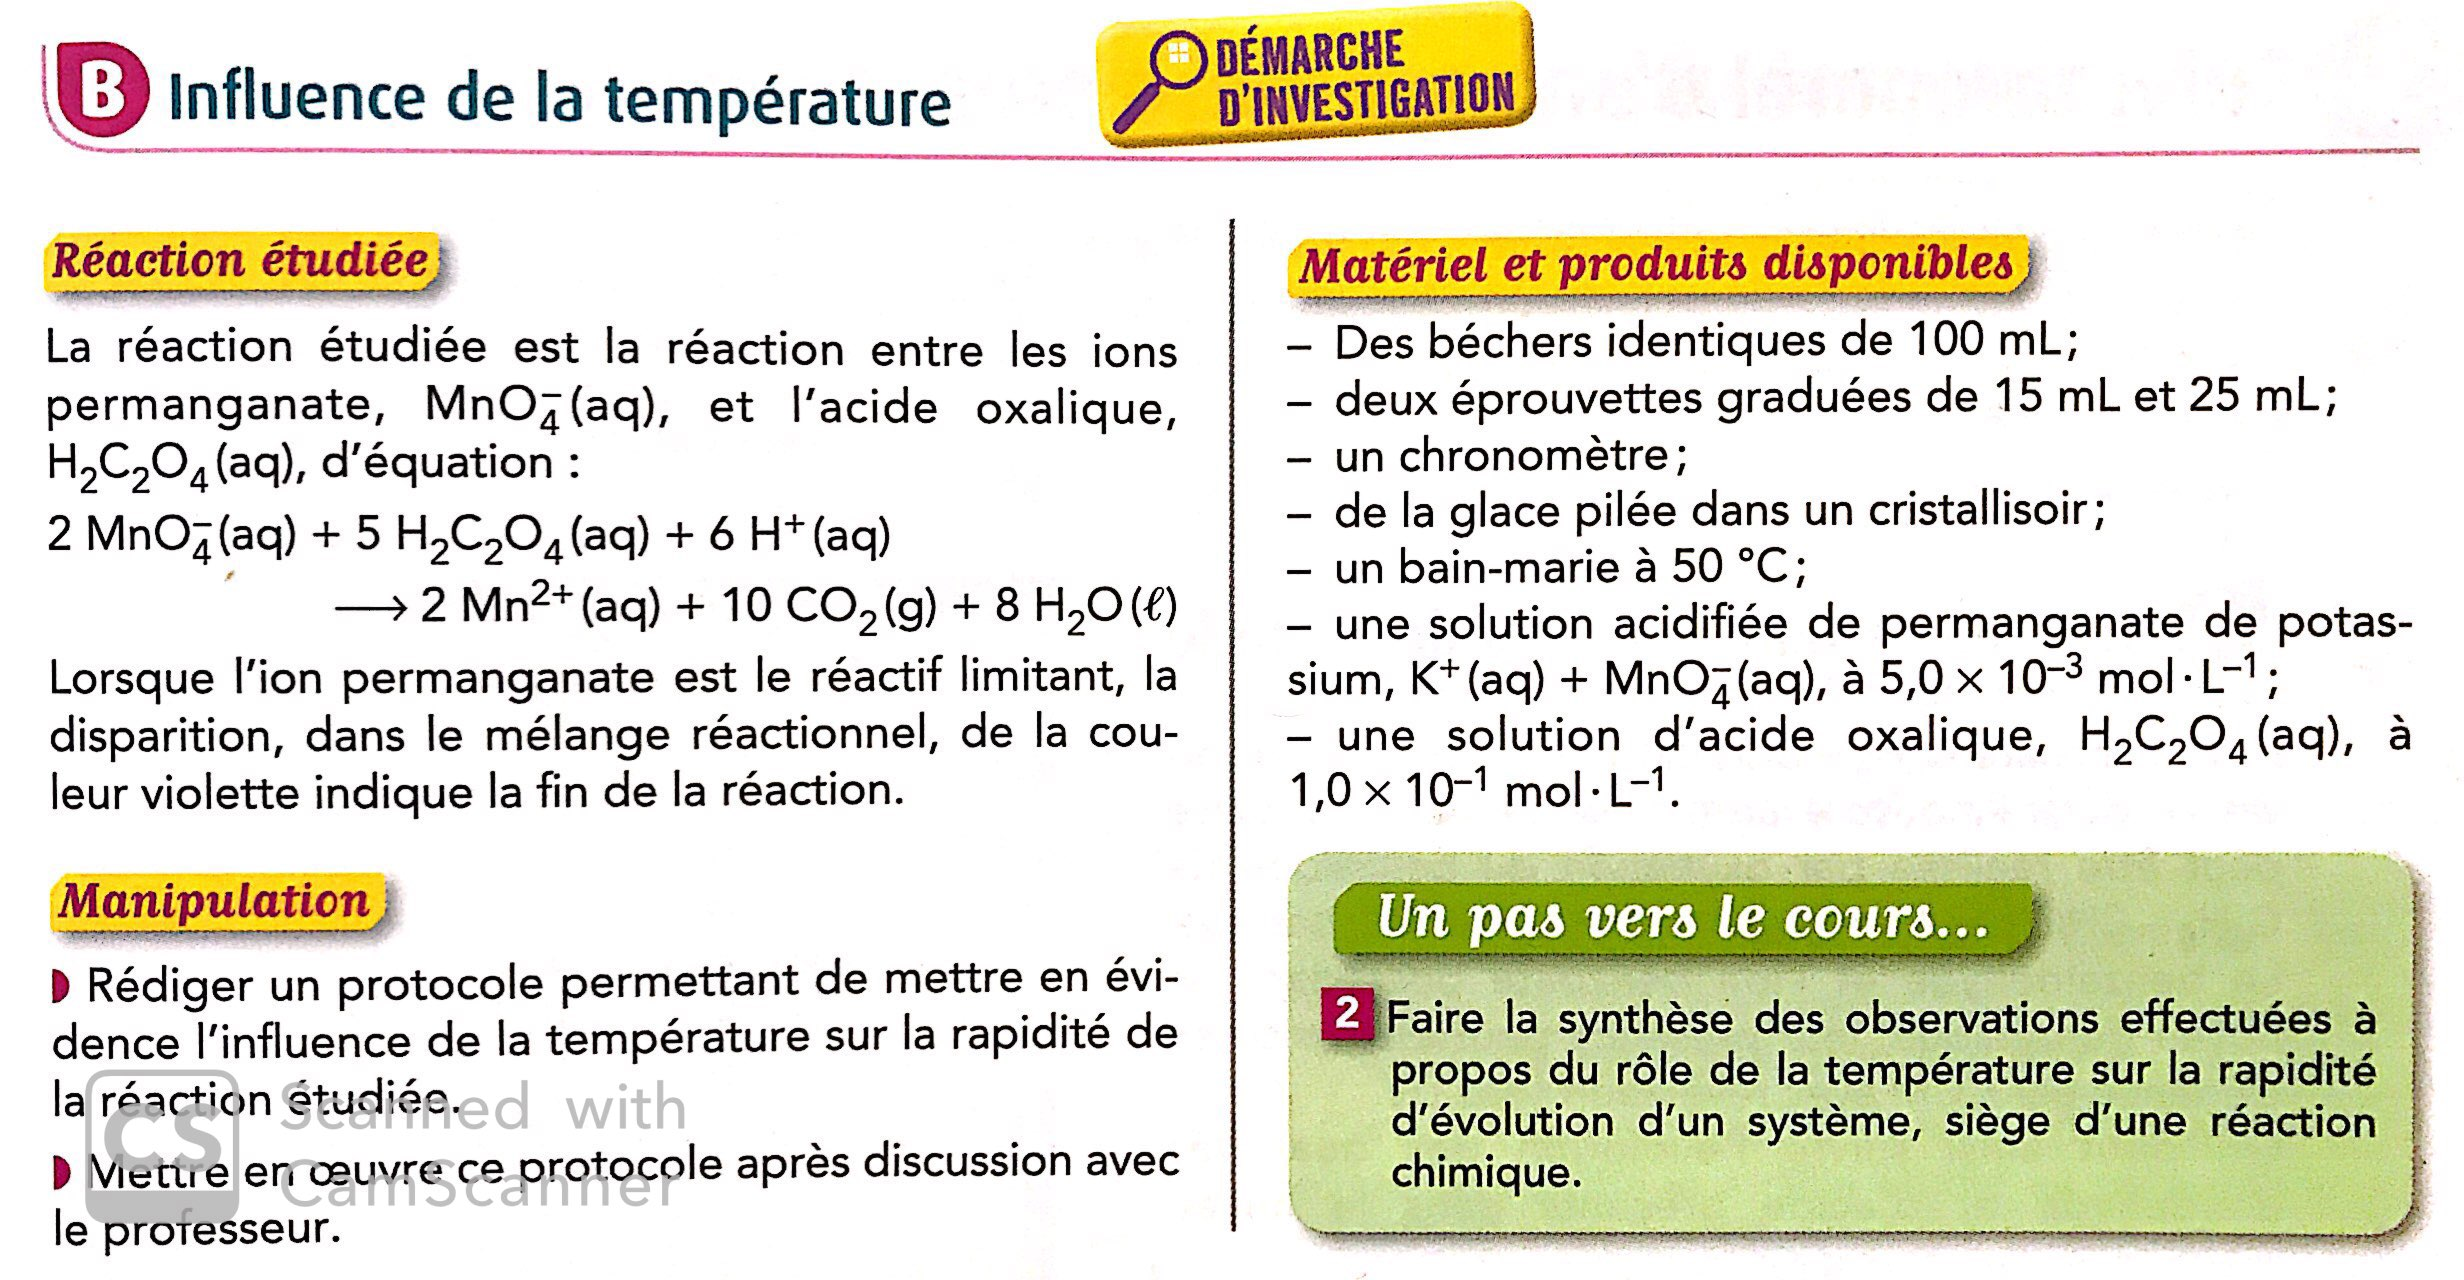
\includegraphics[scale=0.15]{influencetemp.jpg}
\end{center}

\textbf{Conclusion.} Quand la température augmente, la durée de la réaction est réduite. Au contraire, si on refroidit, on freine la réaction. Un refroidissemnt brutal peut même bloquer la réaction (on parle de trempe). La trempe permet de mesurer l'avancement à un instant donné (celui où on a trempé l'échantillon du milieu réactif). : on peut doser le produit sans que les concentrations soient faussées par la réaction. (C'est ce qu'il se passe quand on congèle les aliments, les réactions qui les rendent impropres à la consommation sont bloquées).\\

\textcolor{red}{On peut interpréter microscopiquement nos deux conclusions.} Il y a transformation chimique lorsque deux ou plus réactifs se rencontrent. Quand on augmente la température, l'agitation des molécules augmente donc elles se rencontrent plus souvant. Quand on augmente la concentration, il y a plus de réactifs par unité de volume donc les molécules se rencontrent plus souvant aussi.\\

Il y a aussi \textbf{d'autres facteurs cinétiques} comme le solvant(en chimie orga SN1,SN2...) ou l'éclairement (electron qui monte dans un état antiliant, on monte d'un état singuliet à un état triplet, il a gagné de l'énergie donc réaction plus rapide, par exepmle : synthèse chlorophylienne ou photosynthèse : chez les plantes vertes et certaines bactéries, procesus de fabrication de matière organique à partir de l'eau et du gaz carbonique de l'atmosphère , utilisant la lumière solaire comme source d'énergie et qui produit un dégagement de dioxygène, ce sont des réactions photochimiques). La réaction de photosynthèse est catalysée (regarder document envoyé par JB.\\


\textcolor{red}{Faire lien avec chimie durable}
Les méthodes cinétiques étudiés sont coûteux car il faut chauffer, augmenter la quantité des réactifs... Il existe encore un autre moyen d'augmenter la vitesse d'une réaction. La catalyse.

\section{Catalyse}

\textbf{Définition.} Un catalyseur est une espèce chimique différente des réactifs, dont la présence diminue la durée de la réaction chimique. Il réagit avec les réactifs mais est intégralement régénéré en fion de réaction. Il n'apparaît donc pas dans l'équation bilan et est réutilisable.\\

Un catalyseur ne modifie pas la thermodynamique d'une réaction. Si la réaction est impossible thermodynamiquement, ajouter le catalyseur ne va pas faire demarrer la réaction (il faut catalyseur \textbf{plus} lumière par exemple). Le catalyseur ne modifie que le "chemin réactiuonnel" d'une réaction (il abaisse les énergies de transition), l'état initial est final sont les mêmes. la réaction est donc accélérée, l'état final est atteint plus rapidement.\\


\begin{center}
    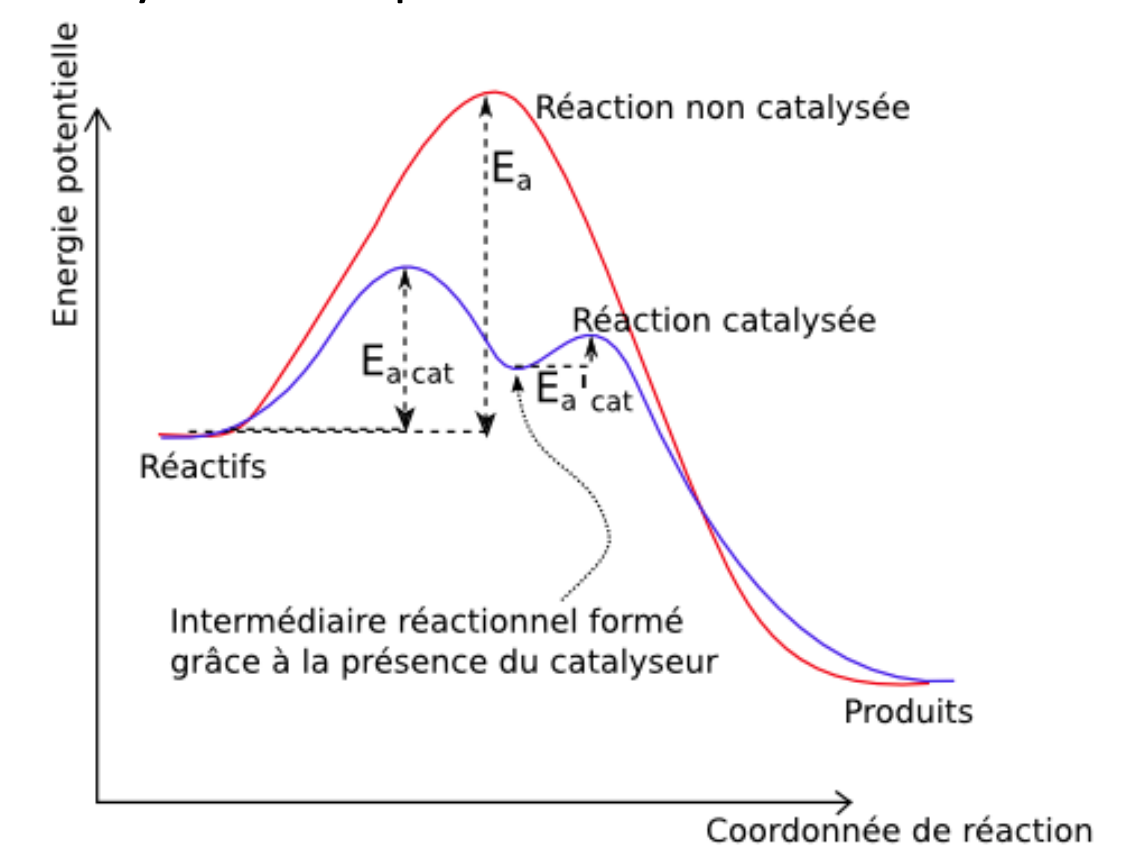
\includegraphics[scale=0.4]{profil_cata.png}
\end{center}

Dans le cas de ce graphique, il y a création d'un intermédiaire réactionnel à cause du catalyseur. Il pourrait ne pas en avoir et juste avoir une bosse plus basse en énergie (au lieu de deux).

\subsection{Types de catalyse}

\textcolor{red}{Manip qualitative}. \textbf{Livre TS pag 231. Réaction de décomposition du peroxyde d'hydrogène \chemform{H_2 O_2} (présent dans l'eau oxygénée). Expliquer chaque type de catalyse et faire chaque manip juste après.\medskip} 

\begin{itemize}
    \item \textbf{Homogène}. Le catalyseur et les réactifs forment un mélange homogène (même phase). Par exemple nous pouvons nous intéresser à la décomposition de l'eau oxygénée. Le peroxyde d'hydrogène appartient à deux couples redox : \chemform{H_2O_2/H_2O} où il joue le rôle d'oxydant et \chemform{O_2 / H_2O_2} où il joue le rôle de réducteur. L'eau oxygénée ne peut donc pas être stable : elle va se dismuter, selon la réaction :
    
    \begin{chemmath}
        2H_2O_{(aq)} = 2H_2O_{(l)} + O_{2(g)}
    \end{chemmath}
    
    Cette réaction est très lente mais peut être accélérée par catalyse homogèene. Faire manip avec ions \chemform{Fe^{3+}}. Comme on utilise du chlorure de fer, il est mieux d'avoir 3 tubes :
    \begin{itemize}
        \item Tube 1 : De l'eau oxygénée à 20 volumes.
        \item Tube 2 : De l'eau oxygénée à 20 volumes plus chlorure de sodium.
        \item Tube 3 : De l'eau oxygénée à 20 volumes plus chlorure de fer(III).
    \end{itemize}
    
    De cette façon on montre qu'avec les ions chlorure ne se passe rien. C'est la présence des ions ferriques qui accélère la réaction.
    
    \item \textbf{Hétérogène}. Le catalyseur et les réactifs forment un mélange hétérogène (phases différentes). Les catalyseurs sont généralement des solides. Faire la manip avec le petit cylindre de platine, on voit un dégagement gazeux.
    
    \item \textbf{Enzymatique}. Le catalyseur est une protéine, appelée enzyme. Les enzymes présentent des cavités ayant une structire spatiale telle que seuls certains réactifs, de forme adaptée, peuvent s'y fixer, un peu comme une clé dans une serrure. Faire la manip avec le morceau de navet, on voit un dégagement gazeux.
\end{itemize}


\begin{center}
    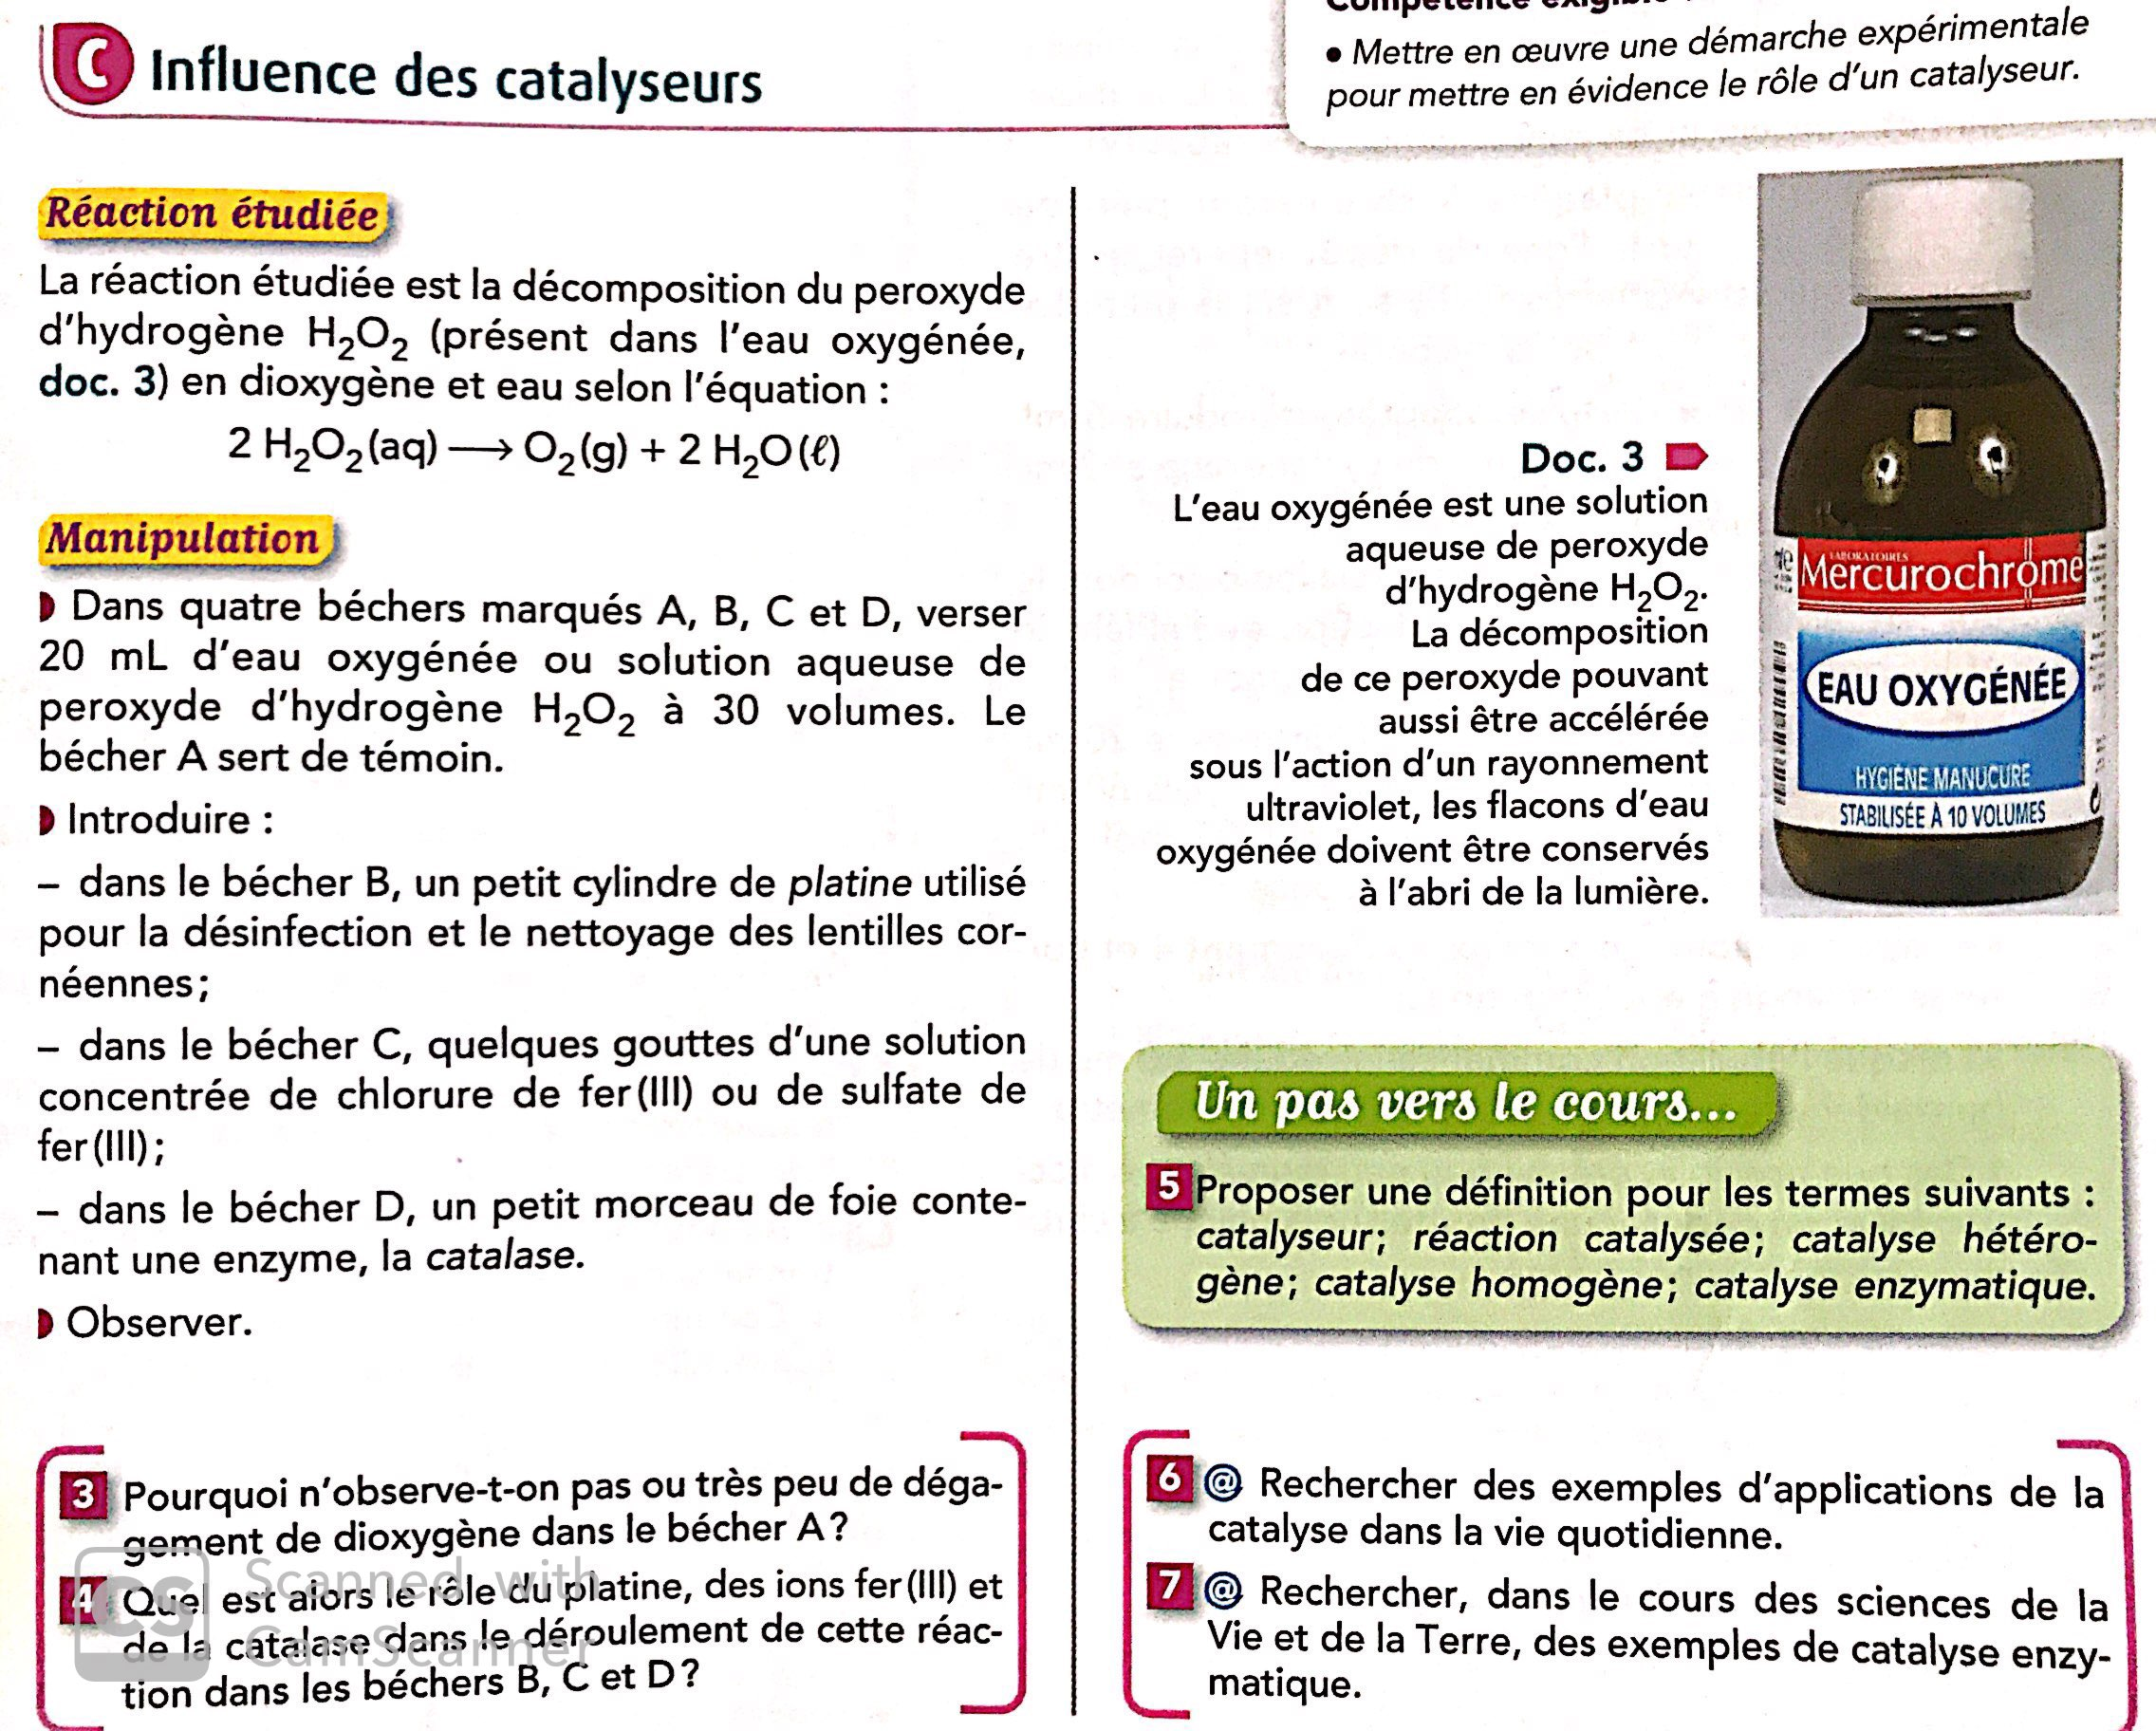
\includegraphics[scale=0.15]{eauoxygene.jpg}
\end{center}


\section*{Conclusion}


\textcolor{red}{Faire le lien avec la chimie durable}\\

Nous avons vu tout au long de cette leçon qu'il est possible de suivre dans le temps l'avancement d'une réaction par des méthodes physiques (mesure de la conductivité, de l'absorbance, CCM) ou chimiques (par trempe plus dosage). Le temps de demi-réaction est une grandeur qui nous permet d'évaluer la rapidité d'une réaction chimique.\\

Nous avons vu qu'il était aussi possible de modifier la vitesse d'une réaction en agissant sur des facteurs comme la température ou la concentartion ou en introduisant un catalyseur dans le milieu. Dans l'industrie, les méthodes catalytiques sont très utilisés, par exemple dans le cas de la \textbf{synthèse de l'ammoniac} (utilisé dans les engrais, entre autres). Cette synthèse serait impossible à échelle industrielle sans catalyseur, car la réaction est très lente. On utilise un catalyseur à base de fer (voir procédé Haber en annexe).\medskip

On peut citer d'autres exemples comme le \textbf{pôt catalytique} des voitures (regarder diapos). Les moteurs à essence rejettent des gaz polluants, résultant du non respect des proportions 	stoechiométriques lors de la combustion des hydrocarbures par le dioxygène : du monoxyde de carbone, des hydrocarbures non brûlés et des oxydes d'azote (\text{NO} et $\text{NO}_2$) sont émis par le moteur. Le pot catalytique a pour objectif de dégrader ces gaz (environ 95\%). Un pot catalytique est constitué d'un isolant thermique en céramique creusé en nid d'abeille, la paroi des alvéoles étant imprégnée de métaux comme le platine (Pt), le rhodium (Rh) et le palladium (Pd). Ces métaux agissent comme catalyseurs dans :
	\begin{itemize}
		\item l'oxydation du monoxyde de carbone en dioxyde de carbone,
		\item la réduction des oxydes d'azote en diazote,
		\item l'oxydation en eau et dioxyde de carbone des hydrocarbures non brûlés par le 						moteur.\\
	\end{itemize}
	\textbf{Remarque :} essence sans plomb nécessaire, car le plomb recouvre les métaux qui ne 		peuvent plus catalyser les réactions. Elles deviennent lentes ou peuvent même être bloquées.\\ 

Finallement, la \textbf{catalyse enzymatique} est très importante en biochimie et en particulier dans le mécanisme de la digestion des médicaments. La digestion est un ensemble de processus mécaniques et chimiques permettant à un organisme 	vivant (nous) de transformer par réaction chimique les aliments consommés (eux) en nutriments assimilables. Divers types de sécrétions digestives (salive, sucs gastrique, pancréatique, intestinal et bile) sont produits par divers organes pour faciliter la digestion. Ces sécrétions contiennent des enzymes chargées de favoriser les réactions chimiques produisant des acides aminés, acides gras, vitamines ... à partir des protides, lipides et glucides (p 296 Physique Chimie Terminale S, Hatier (Nouveau Microméga)).\\
	
	Elles sont particulièrement efficaces : pour briser les liaisons chimiques au sein des protéines sans enzymes, on doit avoir recours à une catalyse par les ions $H^+$ de concentration 6 mol/L à chaud ($110^\circ$C), pendant 24 heures environ, là où la digestion ne dure que quelques heures chez l'être humain.








\newpage
\section*{Annexes}

\subsection*{CCM}

La chromatographie sur couche mince (CCM) est une technique de chromatographie dont la phase mobile est liquide. Elle est couramment utilisée pour séparer des composants dans un but d'analyse (CCM analytique) ou de purification (CCM préparative).\medskip

Elle comprend :

\begin{itemize}
    \item une phase stationnaire : une couche mince de matériel adsorbant (usuellement du gel de silice, de l'oxyde d'aluminium ou de la cellulose)
    \item une phase liquide, dite phase mobile ou éluant : un solvant ou un mélange de solvants qui va entraîner les composés à se séparer le long de la phase stationnaire.
\end{itemize}

\subsubsection*{Rapport frontal}
Le rapport frontal (Rf) ou facteur de rétention d'un composé est le rapport de la distance ligne de dépôt-composé sur la distance ligne de dépôt-front de solvant. Il est compris entre 0 et 1, et est caractéristique du composé, du matériau de la plaque et du système d'éluant.

\subsubsection*{Facteurs influençant la migration}
Le Rf des produits dépend de leur affinité relative pour la phase stationnaire et la phase mobile. Dans la plupart des cas, la phase stationnaire est polaire (silice, alumine, cellulose). Plus un composé est lui-même polaire, plus il aura d'affinité pour la phase stationnaire et, par conséquent, plus il sera retenu sur la plaque. Plus on augmente la polarité de l'éluant, plus il entre en compétition avec la phase stationnaire et puisqu'il est en mouvement, plus il entraîne le composé avec lui.

\rule{\linewidth}{0.2mm}

\subsection*{Synthèse de l'ammoniac}

\textbf{Procédé Haber} : hydrogénation du diazote atmosphérique en présence d'un catalyseur (fer et potasse).
\begin{chemmath}
    N_{2(g)} + 3 H_{2(g)} = 2 NH_{3(g)}
\end{chemmath}
Pour déplacer l'équilibre vers la droite :
\begin{itemize}
	\item augmenter la pression (loi de le Châtelier, une augmentation de la pression déplace l'équilibre dans le sens de la diminution du nombre total de moles de gaz);
	\item maintenir une température faible (loi de Van't Hoff, une augmentation de $T$ déplace l'équilibre vers le sens endothermique, la réaction étant exothermique on doit diminuer $T$);
\end{itemize}

En pratique, la réaction est très lente à basse température (cinétique). Elle se fait donc à une température plus élevée (environ $450^\circ$C) qui permet d'obtenir une quantité appréciable d'ammoniac dans un temps satisfaisant.

\rule{\linewidth}{0.2mm}

\subsection*{Mécanisme probable de formation de la rouille}

Quand le fer entre en contact avec l'eau, un processus électrochimique lent commence, dont les étapes pourraient (c'est apparemment encore une question ouverte) être :\\
\begin{itemize}
	\item \textbf{Etape 1 : oxydation du fer et réduction du dioxygène}
	\begin{equation}
		\text{Fe} + 2\text{OH}^- \rightarrow \text{Fe(OH)}_2 + 2\text{e}^-
	\end{equation}
	\begin{equation}
		2\text{H}_2\text{O} + \text{O}_2 + 4 \text{e}^- \rightarrow 4\text{OH}^-. 
	\end{equation}
	
	\item \textbf{Etape 2 : oxydation de l'hydroxyde de fer(II) en hydroxyde de fer(III)}
	\begin{equation}
		4\text{Fe(OH)}_2 + 2\text{H}_2\text{O} + \text{O}_2\rightarrow 4\text{Fe(OH)}_3 
	\end{equation}	 
	\item \textbf{Etape 3 : formation de l'oxyde de fer(III) hydraté}
	\begin{equation}
		2\text{Fe(OH)}_3 \rightarrow \text{Fe}_2\text{O}_3 + 3\text{H}_2\text{O}.
	\end{equation}
\end{itemize}

\rule{\linewidth}{0.2mm}

\subsection*{Triglyrécides, acides aminés, protéines, glucose}

\subsubsection*{Glycérol et triglycérides}
\begin{figure}[h!]
	\begin{center}
		\begin{tabular}{cc}
  		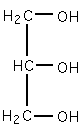
\includegraphics[scale = 1]{glycerol.png} &
   		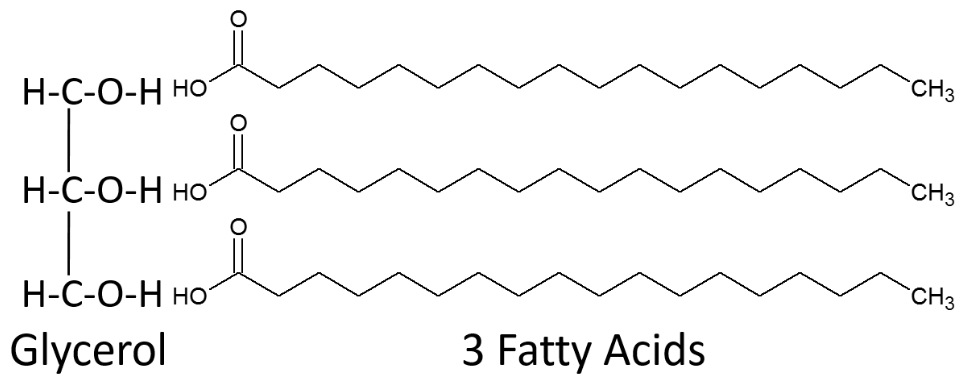
\includegraphics[scale = 0.4]{triglycerides.png}\\
	\end{tabular}
	\caption{Gauche : glycérol. Droite : un triglycéride.}
	\end{center}
\end{figure}

\subsubsection*{Acides alpha-aminés}

\begin{figure}[h!]
	\begin{center}
		\begin{tabular}{cc}
  		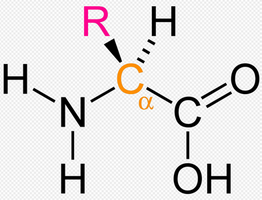
\includegraphics[scale = 0.5]{alpha_amine.png} &
   		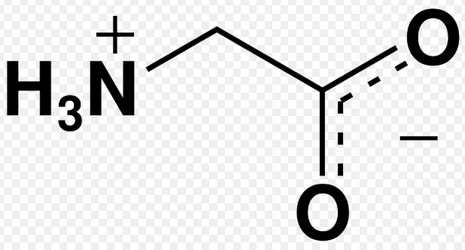
\includegraphics[scale = 0.35]{glycine.png}\\
	\end{tabular}
	\caption{Gauche : forme générale d'un acide $\alpha-$aminé. Droite : la glycine est le plus 			simple d'entre eux, représentée ici sous forme de zwitterion.}
	\end{center}
\end{figure}

Le groupe carboxyle $-\text{COOH}$ est un acide faible, ce qui signifie qu'il tend à libérer un proton pour donner un carboxylate $-\text{COO}^-$ chargé négativement. La forme carboxylate est prédominante à pH supérieur au pKa de l'acide carboxylique, c'est-à-dire environ 2,2 pour les acides aminés protéinogènes. De façon symétrique, le groupe amine $-\text{NH}_2$ est une base faible, ce qui signifie qu'il tend à recevoir un proton pour donner un ammonium $-\text{NH}_3^+$. La forme ammonium prédomine à pH inférieur au pKa de l'amine, c'est-à-dire environ 9,4 pour les acides aminés protéinogènes.

Dans la mesure où, par définition, les acides aminés ont à la fois un groupe carboxyle et un groupe amine, ce sont des molécules amphotères :
\begin{itemize}
	\item $pH < 2,2$, les acides $\alpha$-aminés présentent un groupe carboxyle $-\text{COOH}$ neutre et un groupe ammonium $–\text{NH}_3^+$ chargé positivement, l'ensemble ayant une charge électrique globale $+$1;
	\item $2,2 < pH < 9,4$, les acides $\alpha$-aminés présentent un groupe carboxylate $-\text{COO}^-$ chargé négativement et un groupe ammonium $-\text{NH}_3^+$ chargé positivement, l'ensemble étant globalement neutre (forme zwitterionique);
	\item $pH > 9,4$, les acides $\alpha$-aminés présentent un groupe carboxylate $-\text{COO}^-$ chargé négativement et un groupe amine $-\text{NH}_2$ neutre, l'ensemble ayant une charge électrique globale $-$1.
\end{itemize}

La présence de deux groupes fonctionnels portant des charges électriques opposées $+$1 et $-$1 sur des atomes non adjacents définit un \textbf{zwitterion}. La forme non ionisée des acides aminés est une espèce chimique extrêmement minoritaire en solution aqueuse (moins de 0,1 ppm) puisque généralement au moins l'un des deux groupes est ionisé.\\ 

Pendant la digestion, les acides aminés sont séparés les uns des autres. Vingt d'entre eux environ seront réutilisés par le corps pour fabriquer les protéines des cheveux, de la peau, des muscles, des os, du sang, et d'autres tissus et organes. \textbf{9 acides aminés sont essentiels}, c'est-à-dire que le corps ne peut les synthétiser, et qu'il doit se les procurer dans l'alimentation.

\rule{\linewidth}{0.2mm}

\subsubsection*{Protéines}

Les protéines sont des macromolécules biologiques présentes dans toutes les cellules vivantes. Elles sont formées d'une ou de plusieurs chaînes polypeptidiques. Chacune de ces chaînes est constituée de l'enchaînement de résidus d'acides aminés liés entre eux par des liaisons peptidiques :

\begin{itemize}
	\item \textbf{Liaison peptidique :}
	La liaison est le résultat de la réaction entre la fonction acide carboxylique $\text{COOH}$ du 		premier acide aminé et la fonction amine $\text{NH}_2$ du deuxième, avec comme produit secondaire 	une molécule d'eau.
	\begin{figure}[h!]
		\begin{center}
		\begin{tabular}{cc}
  			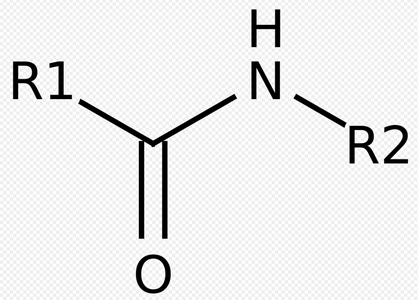
\includegraphics[scale = 0.5]{liaison_peptidique.png} &
   			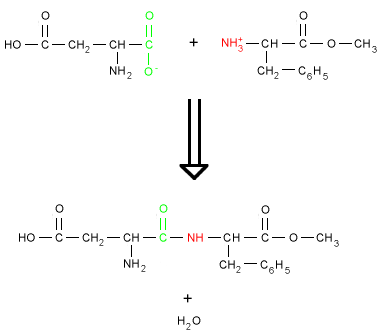
\includegraphics[scale = 0.9]{formation_peptidique.png}\\
		\end{tabular}
		\caption{Gauche : forme générale d'un acide $\alpha-$aminé. Droite : la glycine est le plus 			simple d'entre eux, représentée ici sous forme de zwitterion.}
		\end{center}
	\end{figure}
	
	\item \textbf{Structure des protéines :} quatre niveaux d'organisation
	\begin{itemize}
		\item \textbf{Structure primaire} : séquence en acides aminés;
		\item \textbf{Structure secondaire} : arrangement locaux des acides aminés, 								\textbf{stabilisées par des liaisons hydrogène}, hélices $\alpha$ et feuillets $\beta$;
		\item \textbf{Structure tertiaire} : forme générale de la protéine observable à l'échelle de 				la molécule tout entière (repliement d'une protéine);
		\item \textbf{Structure quaternaire} : complexe résultant de l'assemblage de plusieurs 						molécules de protéines (plusieurs chaînes polypeptidiques), appelées dans ce cas sous-					unités protéiques, pour former un complexe protéique unique. Toutes les protéines ne sont 			pas nécessairement constituées de plusieurs sous-unités et ne possèdent par conséquent 					pas toujours de structure quaternaire.
	\end{itemize}
\end{itemize}

\subsubsection*{Glucose}
\begin{figure}[h!]
	\begin{center}
  		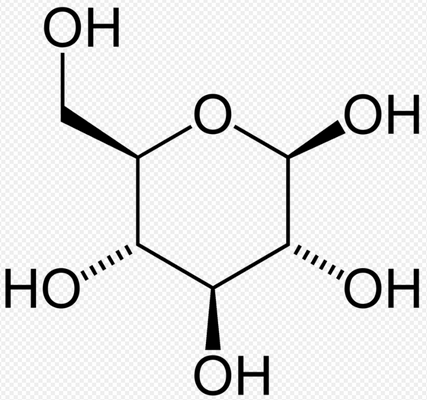
\includegraphics[scale = 0.4]{glucose.png}
	\caption{Glucose.}
	\end{center}
\end{figure}



\end{document}

